%%%%%%%%%%%%%%%%%%%%%%%%%%%%%%%%%%%%%%%%%%%%%%%%%%%%%%%%%%%%%%%%%%%%%%
% writeLaTeX Example: A quick guide to LaTeX
%
% Source: Dave Richeson (divisbyzero.com), Dickinson College
% 
% A one-size-fits-all LaTeX cheat sheet. Kept to two pages, so it 
% can be printed (double-sided) on one piece of paper
% 
% Feel free to distribute this example, but please keep the referral
% to divisbyzero.com
% 
%%%%%%%%%%%%%%%%%%%%%%%%%%%%%%%%%%%%%%%%%%%%%%%%%%%%%%%%%%%%%%%%%%%%%%
% How to use writeLaTeX: 
%
% You edit the source code here on the left, and the preview on the
% right shows you the result within a few seconds.
%
% Bookmark this page and share the URL with your co-authors. They can
% edit at the same time!
%
% You can upload figures, bibliographies, custom classes and
% styles using the files menu.
%
% If you're new to LaTeX, the wikibook is a great place to start:
% http://en.wikibooks.org/wiki/LaTeX
%
%%%%%%%%%%%%%%%%%%%%%%%%%%%%%%%%%%%%%%%%%%%%%%%%%%%%%%%%%%%%%%%%%%%%%%

\documentclass[10pt,landscape]{article}
\usepackage{amssymb,amsmath,amsthm,amsfonts}
\usepackage{multicol,multirow}
\usepackage{calc}
\usepackage{ifthen}
\usepackage{graphicx}
\usepackage{listings}
\usepackage{fancyvrb}
\usepackage[landscape]{geometry}
\usepackage[colorlinks=true,citecolor=blue,linkcolor=blue]{hyperref}


\ifthenelse{\lengthtest { \paperwidth = 11in}}
    { \geometry{top=.3in,left=.3in,right=.3in,bottom=.3in} }
  {\ifthenelse{ \lengthtest{ \paperwidth = 297mm}}
    {\geometry{top=1cm,left=1cm,right=1cm,bottom=1cm} }
    {\geometry{top=1cm,left=1cm,right=1cm,bottom=1cm} }
  }
\pagestyle{empty}
\makeatletter
\renewcommand{\section}{\@startsection{section}{1}{0mm}%
                                {-1ex plus -.5ex minus -.2ex}%
                                {0.5ex plus .2ex}%x 
                                {\normalfont\normalsize\bfseries}}
\renewcommand{\subsection}{\@startsection{subsection}{2}{0mm}%
                                {-1explus -.5ex minus -2ex}%
                                {0.2ex plus -1ex}%
                                {\normalfont\small\bfseries}}
\renewcommand{\subsubsection}{\@startsection{subsubsection}{3}{0mm}%
                                {-1ex plus -.5ex minus -.5ex}%
                                {0.2ex plus -1ex}%
                                {\normalfont\footnotesize\bfseries}}
\makeatother
\setcounter{secnumdepth}{0}
\setlength{\parindent}{0pt}
\setlength{\parskip}{0pt plus 0.5ex}
\graphicspath{ {./images/} }
% -----------------------------------------------------------------------

\title{CS2106 Cheatsheet Finals AY2023/2024 Semester 2}

\begin{document}

\raggedright
\footnotesize

\begin{center}
     \Large{\textbf{CS2106 Cheatsheet Finals AY2023/2024 Semester 2}} \\
\end{center}
\begin{multicols}{3}
\setlength{\premulticols}{1pt}
\setlength{\postmulticols}{1pt}
\setlength{\multicolsep}{1pt}
\setlength{\columnsep}{2pt}
\begin{scriptsize}

\section*{Synchronization}
\subsection*{Properties of CS}
\begin{itemize}
  \item \textbf{Mutual Exclusion} - If a process is within the CS, all other processes are prevented from entering the CS.
  \item \textbf{Progress} - If no process is in the CS, one of the waiting processes should be granted access.
  \item \textbf{Bounded Waiting} - After a process requests to enter the CS< there exists an upper-bound of number times other processes can enter the CS before the requesting process.
  \item \textbf{Independence} - The execution of one process in the CS should not affect/block the execution of another process.
\end{itemize}

\subsection*{TestAndSet Register, MemoryLocation}
\begin{itemize}
  \item Load the current content at MemoryLocation into Register
  \item Set MemoryLocation to 1
  \item EnterCS(int *Lock) \{ while (TestAndSet(Lock) == 1) \}
  \item ExitCS(int *Lock) \{ *Lock = 0; \}
\end{itemize}

\subsection*{Semaphores}
\begin{itemize}
  \item \textbf{Wait(S)} \\ If S $\leq$ 0, block the process. Else, decrement S.
  \item \textbf{Signal(S)} \\ Increment S. Unblock a sleeping process.
  \item Imagine list of waiting process.
  \item $S_{current} = S_{initial} - \text{num of processes in CS}$
  \item $\text{num of processes in CS} = \#Signal(S) - \#Wait(S)$
  \item General Semaphores can be mimicked using binary Semaphores. S = 0, T = 1.
  \item generalWait() - if n == 0 then wait(t); wait(s); n--; signal(s)
  \item generalSignal() - wait(s); n++; signal(s); signal(t)
\end{itemize}

\subsection*{Producer Consumer}
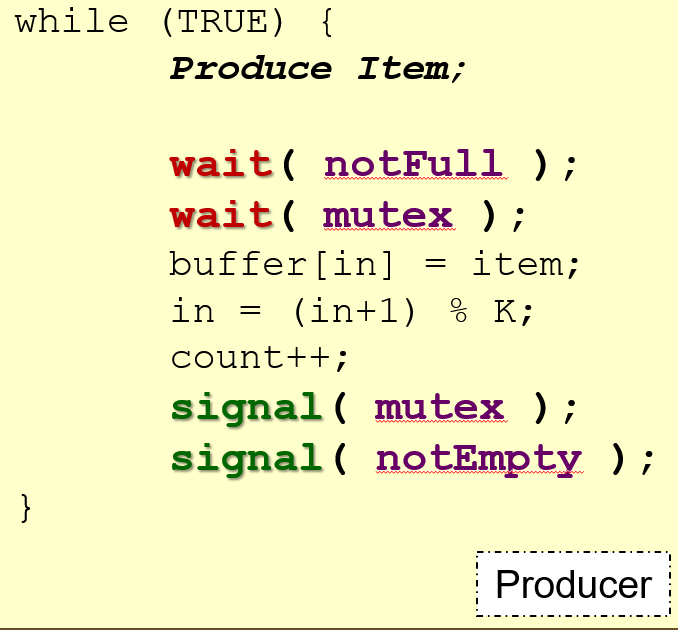
\includegraphics[height= 3cm, width=0.4\linewidth]{producer.png}
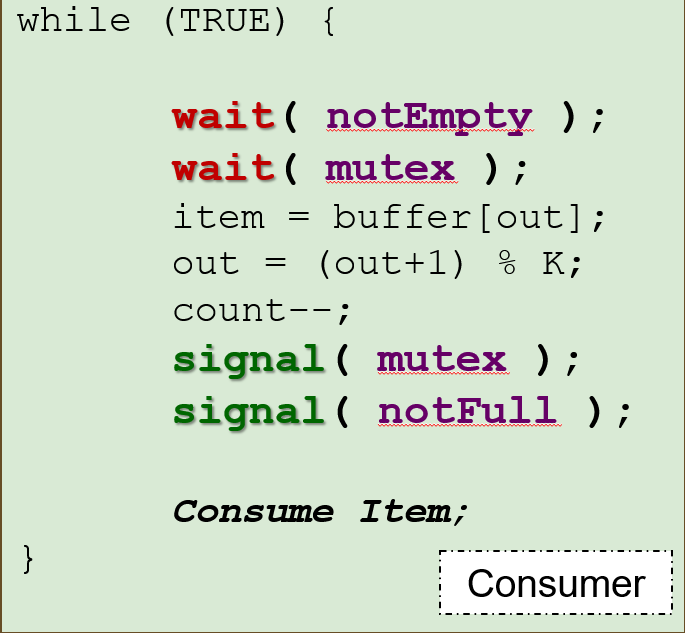
\includegraphics[height= 3cm, width=0.4\linewidth]{consumer.png}\\
busy waiting, canProd, canCons mutexes.

\subsection*{Writer Reader}
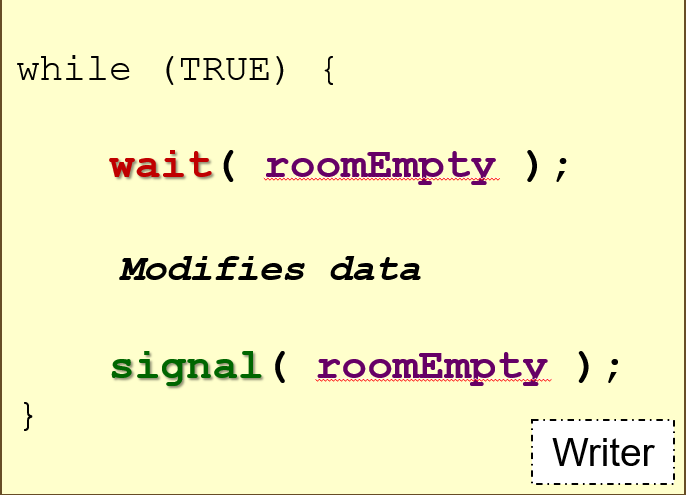
\includegraphics[height= 3cm, width=0.4\linewidth]{writer.png}
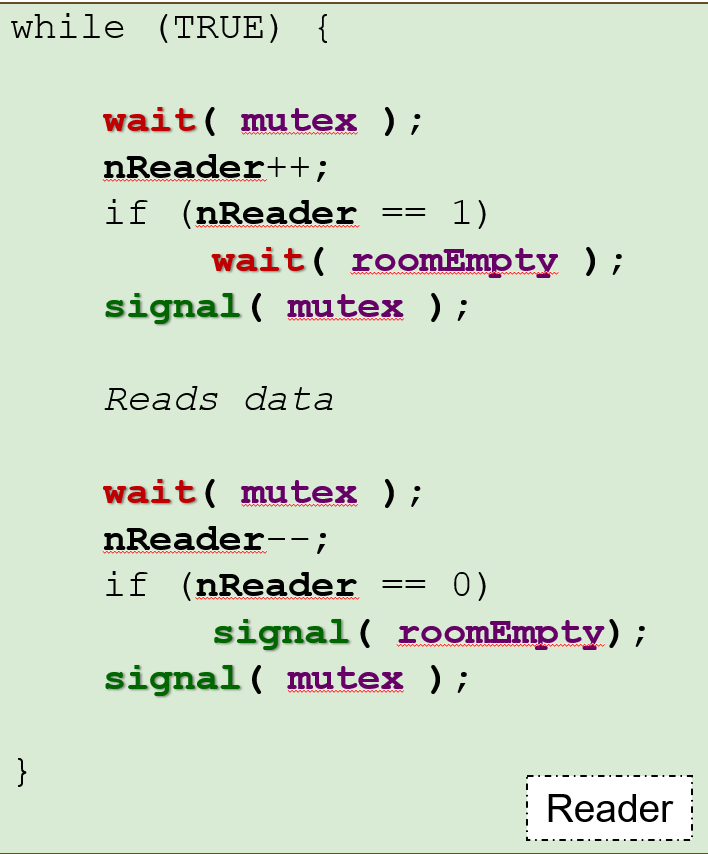
\includegraphics[height= 3cm, width=0.4\linewidth]{reader.png}\\
Potential starvation for writers.

\subsection{Tannenbaum's Solution}
\includegraphics*[height= 3cm, width=0.4\linewidth]{philosopher.png}
\includegraphics*[height= 3cm, width=0.4\linewidth]{takechpstck.png}
\includegraphics*[height= 3cm, width=0.4\linewidth]{saftetoeat.png}
\includegraphics*[height= 3cm, width=0.4\linewidth]{putchpstck.png}
\includegraphics*[height= 3cm, width=0.4\linewidth]{limitedeater.png}

\section{Memory Management}
\subsection*{Continuous Memory Management}
\textbf{Memory Partitioning}\\
\begin{itemize}
  \item Fixed-size partitioning. Internal Fragmentation. Partition Size need to be large enough to hold largest process.
  \item Variable-size partitioning. External Fragmentation. Flexible. Hole Merging. Compaction. Additional bookkeeping.
\end{itemize}
\textbf{Dynamic Partitioning Algo} - First Fit, Best Fit, Worst Fit, Next Fit. Merge when there are adjacent holes .\\

\subsubsection*{Buddy System}
\begin{itemize}
  \item Array of linked lists of free blocks of size $2^{index}$ indicated by start address.
  \item \textbf{Allocate} - Find smallest block that fits. If present, remove from list. If not, find smallest larger free block to split.
  \item \textbf{Free} - Add block to free list. Check buddy. If buddy is free, merge recursively.
  \item \textbf{Find Buddy} - xxx00... and xxx10... are buddies. Same index-1 bits, different $index^{th}$ bit.
\end{itemize}

\subsection*{Disjoint Memory Management}
\subsubsection*{Paging}
\begin{itemize}
  \item Physical memory divided into fixed-size blocks called frames. (Disjoint)
  \item Logical memory divided into same-size blocks called pages. (Continuous)
  \item Page Table: Index = Page Number, Value = Frame Number. Per Process in PCB.
  \item Physical Address = Frame Number $\cdot$ Page Size + Offset.
  \item Offset bits = $\log_2(\text{Page Size})$. Use remaining bits to find frame from page table.
  \item Potential Internal Fragmentation at last page.
  \item 2 Memory Access - Page Table Access, Memory Access.
  \item TLB - Cache for Page Table. Faster access. | Page\# | Frame\# |
  \item Hardware context. TLB Flush on context switch.
  \item Average Mem Access Time = TLB hit + TLB miss = P(TLB hit) $\cdot$ (TLB access + Mem Access) + P(TLB miss) $\cdot$ (2 * Mem Access).
\end{itemize}

\subsubsection*{Segmentation}
\begin{itemize}
  \item Text, Data, Heap Stack. Each segment has a base and limit register.
  \item Segment table: Index = Segment Number, Value = Base Address, Limit.
  \item $<$Segment Number, Offset$>$ $\rightarrow$ $<$Base + Offset$>$. Check if Offset $\leq$ Limit.
  \item External Fragmentation
\end{itemize}

\subsubsection*{Segmentation with Paging}
\begin{itemize}
  \item Each segment has its own page table.
  \item Segment Table: Index = Segment Number, Value = Page Table Base Address.
  \item Page Table: Index = Page Number, Value = Frame Number.
  \item $<$Segment Number, Page Number + Offset$>$
\end{itemize}

\subsection*{Virtual Memory}
\begin{itemize}
  \item Extended Paging Scheme - Memory Resident. Non-Memory Resident.
  \item Page Fault - Page not in memory. OS loads page from disk.
  \item Demand Paging - Only load pages when needed.
\end{itemize}

\subsubsection{Page Table Structure}
\begin{itemize}
  \item Page Table takes up memory. Large page table for large address space.
  \item Number of pages = $\frac{2^{\text{Virtual Address Bits}}}{\text{Page Size}}$
  \item Size of page table = Number of pages $\cdot$ Page Table Entry Size
  \item Branch Factor = $\frac{\text{Page Size}}{\text{PTE Size}}$
  \item Inverted Page Table (Reverse Mapping) - Index = Frame Number, Value = Process ID, Page Number. Auxilary Structure. Linear Scan. Size = Number of Frames $\cdot$ PTE Size.
\end{itemize}

\subsubsection{Multi-Level Paging}
\begin{itemize}
  \item Page Directory pointing to chunk of page tables. 2 Level Paging.
  \item $<$Page Directory Index, Page Table Index, Offset$>$
  \item Entries per chunk = $\frac{\text{Page Size}}{\text{PTE Size}}$
  \item 3 Memory Access - Page Directory Access, Page Table Access, Memory Access.
  \item TLB can be used. But TLB miss is more expensive.
\end{itemize}

\subsubsection{Page Replacement Algorithms}
\begin{itemize}
  \item OPT (Belady's Algorithm) - Replace page that will not be used for longest time. Next use time (max).
  \item FIFO - Replace page that has been in memory the longest. Initial arrival time (min).
  \item LRU - Replace page that has not been used for longest time. Last use time (min). Stack. Logical Time Counter
  \item Clock - Circular list. Hand points to page to be replaced. R++ if hit. If R = 0, replace. Else, set R = 0.
\end{itemize}

\subsubsection{Frame Allocation}
\begin{itemize}
  \item Equal Allocation. Proportional Allocation
  \item Local Replacement (Local Thrashing). Global Replacement (Cascading thrashing)
  \item Working Set Model - $\Delta$ = Time Interval. $WSS_i$ = Working Set Size. $\tau$ = $\Delta$.
\end{itemize}

\section{File System}
Self-Contained, Persistent, Efficient.
\subsubsection{MetaData}
\begin{itemize}
  \item Name. File Extension
  \item Type. Regular File (ASCII, Binary), Directory, Special File (Device, Pipe, Character/Block oriented)
  \item Protection. RWX for Owner, Group, Public. \textit{chmod 760 example.txt}
  \item Structure. Array of Bytes. Fixed Length Records. Variable Length Records. Tree.
\end{itemize}

\subsubsection{Data Access}
\begin{itemize}
  \item Sequential Access. (Contiguous $\rightarrow$ Linked List $\rightarrow$ Indexed)
  \item Random Access.(Contiguous $\rightarrow$ Indexed $\rightarrow$ Linked List) | Read(offset), Seek(offset), bytes.
  \item Direct Access (Fixed Length Records, Random Access on Records)
  \item Operations: Create, Open, Read, Write, Reposition, Truncate, Close
  \item open("file.txt", O\_RDONLY | O\_CREAT, 0644). Returns file descriptor,fd (int).
  \item read(fd, buffer, size). write(fd, buffer, size). close(fd).
\end{itemize}

\subsubsection{File Information}
\begin{itemize}
  \item File Pointer, File Descriptor, Disk Location, Reference Count
  \item Per-Process Open File Table (In PCB, File Descriptor Table, Points to System-wide Open File Table)
  \item System-wide Open File Table (Points to Inode Table)
  \item Inode Table (Points to Data Blocks)
  \item 0 stdin, 1 stdout, 2 stderr. Redirect pointers with dup2(oldfd, newfd).
  \item Different Process opening the same file have different fd, different system-wide open file table entry, same inode table entry.
  \item Parent Child Process. Different fd, same system-wide open file table entry, same inode table entry.
\end{itemize}

\subsubsection{Directory}
\begin{itemize}
  \item Single Level Directory (All files in one directory)
  \item Tree-Structured Directory (Hierarchical, has subdirectories)
  \item Directed Acyclic Graph Directory (Multiple parents, Hard Link: Pointers to same inode, hard delete when reference count = 0)
  \item General Graph Directory (Cycles, Soft Link: Special Link File with pathname to original file, soft delete when file name is deleted)
\end{itemize}

\section*{File System Implementation}
\includegraphics*[height= 3cm, width=0.8\linewidth]{generaldiskorg.png}\\
OS Boot Code: Loads OS into RAM. Partition Details: Free Disk Block Management. Directory Structure. Files Info: Metadata. File Data (File Content).

\subsubsection{File Data}
\begin{itemize}
  \item Contiguous: (Start address, size). Fast. External Fragmentation. File Size $\leq$ Disk Size.
  \item Linked List: (Start address, pointerNext, end address). No External Fragmentation. Slow. Pointer overhead.
  \item Indexed: (Block Location, Index Block Sequence). Index Block: Array of pointers to data blocks. No External Fragmentation. Fast. Index Block[N] Nth Block Address. 
      \\Extensions: Linked List of index blocks, Multi-level index, Combined Scheme (direct indexing + multi-level indexing)
  \item File Allocation Table (FAT): Index: Block Number, Value: Next Block Number. -1 = EOF. Can have empty entries. Entries: FREE, Block Num, EOF, BAD. 
  \item FAT16: $2^{16}$ data blocks in disk. $2^{16}$ FAT Entries. Each entry is 16 bits.
  \item FAT is loaded into RAM, Faster Random Access.
\end{itemize}

\subsubsection{Ext2 File System, I-Node}
\includegraphics*[height= 4cm, width=0.8\linewidth]{ext2inode.png}\\
- 12 Direct Blocks. 1 Single Indirect Block. 1 Double Indirect Block. 1 Triple Indirect Block.\\
- Fast access to small files. Flexibility in handling big files.\\
- Direct = 12 * Block Size.\\
- Num of Entries = Block Size in bytes / bytes of block address.\\
- Single Indirect = Num of Entries * Block Size.\\
- Double Indirect = $\text{Num of Entries}^2 \cdot$ Block Size.\\
- Triple Indirect = $\text{Num of Entries}^3 \cdot$ Block Size.\\

\subsubsection{Free Space Management}
\begin{itemize}
  \item Partition Details.
  \item BitMap. 0 = occupied. 1 = free. 1 bit per block. Fast. Space Overhead.
  \item Linked List. Pointer to next free block.
\end{itemize}

\subsubsection*{Directory Structure}
\begin{itemize}
  \item Linear List of Files. (File Name, File Information or pointer to File Information). (File, Start, Length). Linear Search. Cache.
  \item Hash Table. (Hash Value, File Name, File Information(start, length)). Hash Function. Collisions. Hash Table Limited Size.
  \item \includegraphics*[height= 3cm, width=0.8\linewidth]{FAT16dir.png}
  \item \includegraphics*[height= 3cm, width=0.8\linewidth]{ext2dirstructure.png}
  \item Directory Permissions. Think of directories as a file with list of files. RWX. ls (R), cd (X), any changes to the "file list" (renaming, add/delete files) (W). Individual file permissions are not affected.
\end{itemize}

\subsubsection{File Operation Walkthrough}
\textbf{Create} - Use full pathname to locate parent directory, search for filename. Use free space list to find free disk blocks. Add Entry to parent directory.\\
\textbf{Open} - Use full pathname to locate file. Add entry to per-process open file table, link pointers to system-wide file table and I-node table. Return file descriptor.\\

\subsubsection{open(fd) and fork() behaviour}
File opened before fork(). Child inherits file descriptor. If both parent and child read, both move pointer and result is undeterministic.\\
File opened after fork(). Parent and child have different file descriptors. Each read their own number of bytes.\\
File opened before fork(), but buffer has read 50 words before fork(). After fork(), buffer is copied, both parent child read same 50 bytes, afterwards all undeterministic.\\
File opened before fork(). If read is done using buffer, buffer size number of bytes are not interleaved.

\end{scriptsize}

\end{multicols}

\end{document}